% ****** Start of file adler-2025.tex ******
%
%   This file is part of the APS files in the REVTeX 4.2 distribution.
%   Version 4.2a of REVTeX, December 2014
%
%   Copyright (c) 2014 The American Physical Society.
%
%   See the REVTeX 4 README file for restrictions and more information.
%
% TeX'ing this file requires that you have AMS-LaTeX 2.0 installed
% as well as the rest of the prerequisites for REVTeX 4.2
%
% See the REVTeX 4 README file
% It also requires running BibTeX. The commands are as follows:
%
%  1)  latex apssamp.tex
%  2)  bibtex apssamp
%  3)  latex apssamp.tex
%  4)  latex apssamp.tex
%
\documentclass[%
 preprint, linenumbers,
%superscriptaddress,
%groupedaddress,
%unsortedaddress,
%runinaddress,
%frontmatterverbose, 
%preprint,
%preprintnumbers,
%nofootinbib,
%nobibnotes,
%bibnotes,
 amsmath,amssymb,
 aps, physrev,
%pra,
%prb,
%rmp,
%prstab,
%prstper,
%floatfix,
]{revtex4-2}

\usepackage{graphicx}% Include figure files
\usepackage{dcolumn}% Align table columns on decimal point
\usepackage{bm}% bold math
%\usepackage{hyperref}% add hypertext capabilities
%\usepackage[mathlines]{lineno}% Enable numbering of text and display math
%\linenumbers\relax % Commence numbering lines

%\usepackage[showframe,%Uncomment any one of the following lines to test 
%%scale=0.7, marginratio={1:1, 2:3}, ignoreall,% default settings
%%text={7in,10in},centering,
%%margin=1.5in,
%%total={6.5in,8.75in}, top=1.2in, left=0.9in, includefoot,
%%height=10in,a5paper,hmargin={3cm,0.8in},
%]{geometry}

\begin{document}

\preprint{APS/123-QED}

\title{\textbf{Information Evolution Dynamics} 
}% 


\author{Dan Adler}
\email{dan@danadler.com}
\date{\today}% It is always \today, today,
             %  but any date may be explicitly specified

\begin{abstract}
The emergence of complexity from simple interactions is a fundamental question in the study of dynamical systems. In this paper, we develop a formal framework to analyze Information Evolution Dynamics in abstract ABC systems, extending earlier work that modeled the evolution of stable information structures. We introduce a graph-based representation of ABC systems, where the base elements and compounds flow through networks of nodes and edges with stability constraints, analogous to resistance-capacitance (RC) circuits, fluid dynamics, and the economic principles of supply and demand. By analyzing these flows, we reveal how the system exhibits emergent resource allocation, self-organization, and path-dependent evolution.

We further derive a Lagrangian formulation of ABC dynamics, demonstrating that the system evolves according to the principle of least action in the continuum limit. Optimal transport analysis illustrates how efficient redistribution of resources emerges without requiring intelligent agents, providing new insights into economic and ecological systems. Finally, we link these dynamics to Rube-Goldberg machines, autocatalytic sets, and dynamic control mechanisms, showing how complexity arises through simple interactions constrained by stability. These results underscore the universality of ABC systems in modeling emergent phenomena and their potential to unify diverse dynamical systems.
\end{abstract}

%\keywords{Suggested keywords}%Use showkeys class option if keyword
                              %display desired
\maketitle

%\tableofcontents

\title{Information Evolution Dynamics}

\author{Your Name}
\affiliation{Your Institution}

\maketitle

\section{Introduction and Background}

The emergence of complexity and information from randomness is a profound question spanning physics, biology, chemistry, and computation. Traditional approaches, such as Lloyd's computational perspective in \textit{Programming the Universe} \cite{lloyd2006programming}, Davies' exploration of information's role in biological processes in \textit{The Demon in the Machine} \cite{davies2019demon}, Tegmark's "Mathematical Universe" \cite{tegmark2008mathematical}, and Wolfram's computational universe framework \cite{wolfram2020fundamental}, often conceptualize complexity and information as emergent properties. However, these works leave unresolved how such properties arise dynamically from abiotic processes. Building on the framework established in "How Information Evolves" \cite{adler2024howinfoevolves}, this paper extends the principles of evolution to abiotic systems, demonstrating how information can emerge and self-organize through stability-driven selection and probabilistic interactions.

ABC systems provide an abstract, yet powerful framework for exploring these dynamics. By abstracting away specific physical laws, they reveal universal mechanisms for generating patterns, encoding information, and fostering complexity. These systems model the evolution of base elements (\(A, B, C\)) and compounds (\(AB, ABC\)) over successive generations, where stability constraints and interaction probabilities determine the persistence and proliferation of patterns. This iterative process mirrors evolutionary principles but operates in entirely abiotic contexts, illustrating how evolution can act as a unifying framework across disciplines.

Represented as dynamic graphs, ABC systems model the flow of elements and compounds through networks of nodes and edges. Stability constraints govern these flows, analogous to resistances in electrical circuits \cite{nowak2006evolutionary}, pressure gradients in fluid dynamics \cite{landau1987fluid}, and supply-demand dynamics in economics \cite{mascolell1995microeconomic}. The interplay between local interactions and global patterns leads to emergent behaviors such as resource allocation, self-organization, and path-dependent evolution. These dynamics encode computational rules, recursive causality, and even self-replicating behaviors, offering a comprehensive perspective on the transition from disordered states to structured configurations.

To deepen this understanding, we derive a Lagrangian formulation of ABC dynamics, demonstrating that the system evolves according to the principle of least action in the continuum limit \cite{goldstein2002classical}. Furthermore, we employ optimal transport analysis \cite{villani2008optimal} to reveal how efficient redistribution of resources emerges naturally, without the need for intelligent agents. These theoretical insights are complemented by analogies to Rube-Goldberg machines, autocatalytic sets \cite{kauffman1996at}, and dynamic control mechanisms, showing how complexity arises through simple interactions constrained by stability.

By integrating concepts from physical systems, biological evolution, and computational frameworks, this study expands the applicability of evolution to abiotic processes, bridging randomness and complexity. The universality of the ABC framework underscores its potential to unify diverse dynamical systems, from prebiotic chemistry to economic systems and information theory.

\subsection{Core Concepts of ABC Systems}

The foundational principles of ABC systems include:
\begin{enumerate}
    \item \textbf{Base Elements and Compounds:}
    Base elements (\(A, B, C\)) interact to form compounds (\(AB, ABC\)), which persist or decay based on stability constraints. New base elements are added at each generation, sustaining interactions and enabling the continuous evolution of patterns.
    \item \textbf{Longevity and Turnover:}
    Patterns have a characteristic lifespan, disappearing after a fixed number of generations unless reinforced by subsequent interactions. This mechanism introduces dynamic turnover and reflects environmental or intrinsic stability constraints.
    \item \textbf{Stability-Driven Selection:}
    Interaction probabilities are governed by stability values (\(S(i, j)\)), which favor patterns that persist and interact frequently. This creates a feedback loop where stability drives selection and evolution.
\end{enumerate}

These principles enable the modeling of diverse phenomena, from simple patterns to recursive structures such as polysaccharides and autocatalytic sets. Such recursive dynamics introduce higher-order stability, allowing for the emergence of complex information-bearing systems.

\subsection{Expanding on Previous Work}

In "How Information Evolves" \cite{adler2024howinfoevolves}, we introduced ABC systems as a framework for studying the evolution of stable information structures. The focus was on the principles underlying the emergence of complexity, entropy reduction, and resource allocation, linking these to evolutionary dynamics and information theory. This paper extends those ideas by investigating the dynamical aspects of the evolution of information, emphasizing the flow of base elements and compounds through evolving interaction networks.

Key questions addressed in this work include:
\begin{enumerate}
    \item How do resource flows within ABC systems mirror principles from physics (e.g., RC circuits, fluid dynamics) and economics (e.g., supply-demand dynamics)?
    \item How do stability constraints and probabilistic interactions lead to emergent self-organization and efficient resource redistribution?
    \item What insights can a Lagrangian formulation of ABC dynamics provide about the underlying principles governing these systems?
\end{enumerate}

\subsection{Structure of This Paper}

Section II formalizes the mathematical representation of ABC systems, including vector and graph-based models. Section III introduces the dynamic graph framework, focusing on token flows and stability-driven evolution. In Section IV, we derive the Lagrangian formulation, demonstrating how ABC systems evolve according to the principle of least action. Section V explores emergent phenomena, including optimal transport, autocatalytic sets, and dynamic control mechanisms. Finally, Section VI summarizes the findings and discusses future research directions.

This expanded framework offers a new lens for understanding how complexity and information emerge in abiotic systems, providing a pathway to unify the study of diverse dynamical systems across disciplines.

\section{Comparative Analysis of Unrestricted and Stability-Driven Symbolic Evolution}

In this section, we analyze the dynamics of two symbolic evolution systems: the \textit{unrestricted system}, where all pairwise interactions are allowed without constraints, and the \textit{stability-driven system}, where only stable compounds persist. The comparison focuses on state space growth, entropy dynamics, and variability across simulation runs. We derive expressions for the entropy variance in both systems and provide simulation results.

\subsection{Entropy and Variance in the Unrestricted System}

The unrestricted system permits all pairwise interactions among symbols, leading to rapid expansion of the state space. Let \( S(t) \) denote the set of all symbols (base symbols and compounds) at generation \( t \). The total state space \( D(t) \) grows as:
\begin{equation}
    D(t) = D_\text{base} + D_\text{compounds}(t),
\end{equation}
where \( D_\text{base} = k \) (the number of base symbols) and \( D_\text{compounds}(t) \) is the number of unique compounds generated. Each pairwise interaction generates a new compound, resulting in:
\begin{equation}
    D_\text{compounds}(t) \sim \sum_{i=1}^t \binom{N^{(i)}}{2},
\end{equation}
where \( N^{(i)} \) is the total number of symbols at generation \( i \). For large \( t \), this leads to superexponential growth:
\begin{equation}
    D(t) \sim \mathcal{O}(2^t).
\end{equation}

The entropy at generation \( t \) is defined as:
\begin{equation}
    H^{(t)} = -\sum_{s \in S(t)} \frac{n_s^{(t)}}{N^{(t)}} \log \left( \frac{n_s^{(t)}}{N^{(t)}} \right),
\end{equation}
where \( n_s^{(t)} \) is the count of symbol \( s \) at generation \( t \), and \( N^{(t)} = \sum_{s \in S(t)} n_s^{(t)} \) is the total number of symbols.

To compute the variance of entropy across simulation runs, we start with:
\begin{equation}
    \text{Var}(H^{(t)}) = \frac{1}{R} \sum_{r=1}^R \left(H_r^{(t)} - \mathbb{E}[H^{(t)}]\right)^2,
\end{equation}
where \( H_r^{(t)} \) is the entropy of run \( r \), and \( \mathbb{E}[H^{(t)}] = \frac{1}{R} \sum_{r=1}^R H_r^{(t)} \).

The state space \( D(t) \) grows rapidly, leading to large variations in symbol counts \( n_s^{(t)} \) across runs. Small differences in early interactions propagate exponentially, resulting in:
\begin{equation}
    \text{Var}(H_\text{unrestricted}(t)) \sim \mathcal{O}(t^2).
\end{equation}

\subsection{Entropy and Variance in the Stability-Driven System}

The stability-driven system restricts interactions to produce only stable compounds, which persist for longer periods. This introduces regularity in symbol distributions and slows state space growth. The effective state space \( D_\text{effective}(t) \) is:
\begin{equation}
    D_\text{effective}(t) = D_\text{base} + \sum_{i=1}^t p_\text{stable} \binom{N^{(i)}}{2},
\end{equation}
where \( p_\text{stable} \) is the fraction of interactions producing stable compounds. For large \( t \), the growth is sublinear:
\begin{equation}
    D_\text{effective}(t) \sim \mathcal{O}(t^k), \quad k < 2.
\end{equation}

The entropy in this system is:
\begin{equation}
    H^{(t)} = -\sum_{s \in S_\text{effective}(t)} \frac{n_s^{(t)}}{N^{(t)}} \log \left( \frac{n_s^{(t)}}{N^{(t)}} \right).
\end{equation}

Variability in \( n_s^{(t)} \) is minimized due to the decay of unstable compounds and the bias towards stable interactions. For the stability-driven system:
\begin{equation}
    \text{Var}\left(\frac{n_s^{(t)}}{N^{(t)}}\right) \sim \mathcal{O}\left(\frac{1}{t}\right).
\end{equation}
Summing over the effective state space, the entropy variance becomes constant:
\begin{equation}
    \text{Var}(H_\text{stability}(t)) \sim \mathcal{O}(1).
\end{equation}

The following table summarizes the differences:

\begin{table}[h!]
\caption{Comparison of Unrestricted and Stability-Driven Symbolic Evolution Dynamics}
\label{tab:comparison}
\begin{ruledtabular}
\begin{tabular}{lcc}
\textbf{Property} & \textbf{Unrestricted System} & \textbf{Stability-Driven System} \\ \hline
\textbf{State Space Growth} & $D(t) \sim \mathcal{O}(2^t)$ & $D_\text{effective}(t) \sim \mathcal{O}(t^k), k < 2$ \\ 
\textbf{Entropy} & $H^{(t)} \sim \log D(t)$ & $H^{(t)} \to H_\text{max}$ \\ 
\textbf{Entropy Variance} & $\text{Var}(H^{(t)}) \sim \mathcal{O}(t^2)$ & $\text{Var}(H^{(t)}) \sim \mathcal{O}(1)$ \\ 
\textbf{Interaction Rules} & All pairwise interactions & Restricted to stable compounds \\ 
\textbf{Symbol Distributions} & Path-dependent and broad & Regular and constrained \\ 
\textbf{Effect of Early Interactions} & Exponential divergence & Minimal long-term impact \\
\end{tabular}
\end{ruledtabular}
\end{table}


\subsection{Monte Carlo Simulations and Results}

To validate these derivations, we performed Monte Carlo simulations for both systems over \( R = 100 \) runs, each with \( T = 30 \) generations and \( k = 5 \) base symbols. Entropy was computed at each generation, and its variance across runs was measured. The simulation results confirm the theoretical predictions: the entropy variance in the unrestricted system grows quadratically, while the stability-driven system exhibits bounded variance.

\begin{figure}[h]
    \centering
    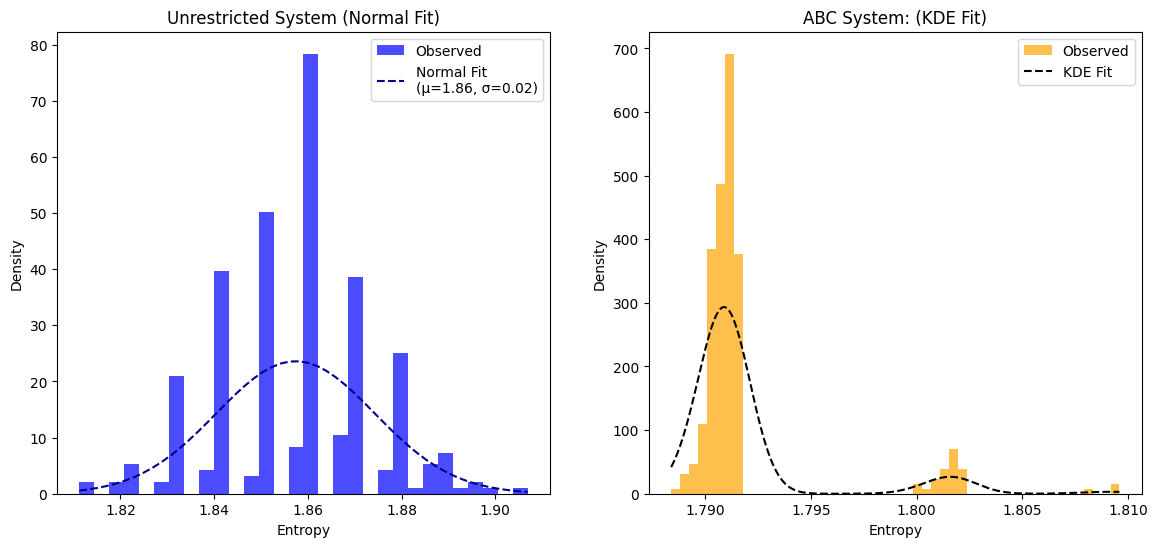
\includegraphics[width=1\linewidth]{monte-carlo-fits.png}
    \caption{Comparison of entropy variance across generations for unrestricted (blue) and stability-driven (orange) systems. The unrestricted system exhibits quadratic growth in variance, while the stability-driven system remains bounded.}
    \label{fig:entropy_variance}
\end{figure}


\subsection{Probability Distribution}

To gain deeper insight into the relative abundances of patterns, we define a probability distribution $\mathbf{p}_t$ as the normalized form of the population vector $\mathbf{n}_t$:
\begin{equation}
\mathbf{p}_t = \frac{\mathbf{n}_t}{\sum_i n_{i,t}},
\end{equation}
where $n_{i,t}$ represents the count of the $i$th pattern at generation $t$. This distribution evolves alongside the population vector, driven by the same interaction dynamics and stability constraints.

Patterns with higher stability values tend to dominate the probability distribution over time, creating a feedback loop where stability influences persistence and interaction likelihoods. This probabilistic perspective highlights the balance between exploration and exploitation in the system's evolution.

\subsection{Integration of Vector and Graph Frameworks}

The vector and graph-based representations are inherently complementary. The vector framework offers a compact and efficient way to track population dynamics, while the graph framework captures the adaptive topology and interaction pathways that drive the evolution of complexity. Together, they provide a unified view of ABC systems.

By integrating these approaches, we can address key aspects of the behavior of the system. The vector representation ensures the conservation of tokens and facilitates the analysis of population distributions, while the graph representation models the dynamic creation and dissolution of patterns. This dual perspective enables us to explore emergent phenomena such as resource allocation, self-organization, and path-dependent evolution, which are fundamental to understanding the dynamics of ABC systems. The synergy between these frameworks will be further illustrated in subsequent sections, where we examine specific emergent behaviors and their implications for information evolution.

\section{Graph-Based Representation of ABC Systems}

The graph-based representation of ABC systems offers a dynamic and intuitive framework to understand the evolving topology of interactions and patterns. Unlike the vector approach, which focuses primarily on population dynamics, the graph-based model emphasizes the structural and relational aspects of the system. This perspective is essential to capture the stochastic and adaptive nature of ABC systems, where interactions continuously reshape the system's topology.

In this framework, nodes represent the fundamental elements ($A$, $B$, $C$) and the compounds they form (for example, $AB$, $ABC$). The edges between these nodes represent possible interactions, with weights proportional to their stability values $S(i, j)$. As interactions occur, the graph evolves: new nodes and edges are introduced to represent emerging compounds and interactions, whereas existing nodes and edges may disappear as patterns decay. For example, if $A$ and $B$ interact to form $AB$, a new node that represents $AB$ could be added, along with edges connecting it to other relevant nodes such as $C$, allowing subsequent interactions like $AB + C \to ABC$.

The dynamic nature of this topology reflects the probabilistic rules that govern interactions. The nodes and edges are not static; they adapt on the basis of interaction outcomes and stability constraints. This adaptability ensures that the graph captures both exploratory dynamics, where new patterns are tested, and selective dynamics, where stable configurations are reinforced.

The edges of the graph are weighted to reflect the likelihood of interactions between nodes. These weights depend on both the stability of the interaction and the populations of the interacting nodes. Mathematically, the weight of an edge between nodes $i$ and $j$ is given by:
\begin{equation}
W(i, j) = S(i, j) \cdot N(i) \cdot N(j),
\end{equation}
where $S(i, j)$ is the stability value, and $N(i)$ and $N(j)$ are the populations of the respective nodes. High edge weights signify strong interaction probabilities, making associated reactions more likely. As interactions progress, edge weights adjust dynamically to reflect shifts in population distributions and stability conditions.

One of the key advantages of the graph-based approach is its ability to reveal emergent network properties that arise from local interactions. Properties such as connectivity, clustering coefficients, path lengths, and cycle formation provide valuable insights into the system’s organization and its ability to sustain complexity. For example, highly connected nodes and clusters often represent stable regions of the graph where certain patterns dominate. In contrast, sparsely connected regions may indicate exploratory zones where less probable configurations are being tested. Cycles, including autocatalytic loops, are particularly noteworthy as they represent feedback mechanisms that can amplify certain patterns or facilitate their persistence.

Visualization plays a crucial role in interpreting the graph representation. By plotting nodes and edges, one can observe the evolution of the network over generations, identifying clusters, cycles, and highly connected hubs. This visualization highlights the balance between exploration and exploitation. Regions with frequent node turnover correspond to exploratory phases where the system samples new possibilities, while stable clusters indicate zones of exploitation where favorable patterns prevail.

The graph-based representation complements the vector/matrix framework by linking topological changes to population dynamics. The node populations in the vector model correspond directly to the node attributes in the graph, while the interaction probabilities inform the edge weights. This integration provides a dual lens for analyzing the system: the graph captures the relational and structural pathways driving evolution, while the vector/matrix representation quantifies the outcomes of these interactions at a population level. Together, these perspectives offer a comprehensive understanding of how complexity emerges and evolves in ABC systems.

In subsequent sections, we delve deeper into the emergent phenomena that arise from these dynamics, such as autocatalytic cycles, resource bottlenecks, and self-organizing clusters. These features underscore the utility of the graph model in uncovering the principles that govern the evolution and formation of information.

\section{Emergent Phenomena in ABC Systems}

ABC systems are not merely collections of interacting elements; they are dynamic networks that exhibit emergent behaviors shaped by stability constraints, probabilistic interactions, and the interplay between local and global dynamics. These emerging phenomena provide insight into the principles that govern complexity and information evolution. In this section, we explore key emergent features such as resource allocation, autocatalytic cycles, and self-organization, illustrating how these properties arise naturally from the dynamics of ABC systems.

The first striking feature of ABC systems is the emergent allocation of resources across patterns. As base elements and compounds interact, stability-driven selection biases the flow of tokens toward configurations that persist longer or interact more frequently. This dynamic allocation mirrors the economic principles of supply and demand, where resources gravitate toward the most "efficient" configurations under given constraints. For example, if certain patterns such as $AB$ exhibit higher stability, the system will naturally channel resources to maintain and propagate these configurations, even as other patterns fade.

Another prominent phenomenon is the formation of autocatalytic cycles. These are feedback loops in which a set of interactions reinforces its own existence. For example, a compound $AB$ could catalyze the formation of another compound $BC$, which, in turn, promotes the regeneration of $AB$. Such cycles can stabilize regions of the graph and act as hubs of activity, driving the persistence of certain patterns and enabling recursive interactions. This self-reinforcing behavior is reminiscent of the autocatalytic sets observed in chemical and biological systems, providing a bridge between the abiotic and biotic evolutionary dynamics.

Self-organization is also a hallmark of ABC systems. The interplay between local interactions and global patterns leads to the spontaneous emergence of order without central control. Clusters of stable patterns form as localized "islands" of high connectivity within the graph. These clusters often correspond to regions of high stability and interaction frequency, and their formation is a natural consequence of the system’s tendency to exploit favorable configurations while continuing to explore new possibilities. Self-organization in ABC systems demonstrates how complexity can emerge from simple, probabilistic rules.

Visualization of these emergent phenomena provides a powerful tool for understanding the dynamics of ABC systems. By examining how the graph evolves over generations, one can identify transitions from exploratory phases, where new patterns dominate, to exploitative phases, characterized by the reinforcement of stable configurations. The shifting topology reveals the underlying mechanisms that balance randomness and structure, driving the evolution of information and complexity.

These emergent properties also highlight the robustness and adaptability of ABC systems. Resource allocation ensures that the system can efficiently utilize its base elements, while autocatalytic cycles and self-organization allow it to adapt to changing conditions. Together, these phenomena underscore the versatility of ABC systems as models for exploring the dynamics of evolution and complexity in diverse contexts.

In the following sections, we build on this foundation to formalize the principles underlying these emergent behaviors. Through mathematical analysis and numerical simulations, we aim to uncover the deeper mechanisms driving these phenomena and their implications for understanding the evolution of complexity.

\section{Lagrangian Framework for ABC Dynamics}

A deeper understanding of ABC systems can be achieved by analyzing their evolution through the lens of variational principles. By formulating a Lagrangian framework, we establish a connection between the dynamics of ABC systems and the principle of least action, a cornerstone of classical mechanics. This perspective provides a unified way to describe the behavior of the system, focusing on the interaction between stability-driven interactions, probabilistic dynamics, and resource redistribution.

The evolution of an ABC system can be viewed as a process that minimizes a global cost function, analogous to the action in physics. To formalize this, we define a Lagrangian $\mathcal{L}$ that captures the balance between kinetic and potential terms, representing the redistribution of tokens and the stability constraints, respectively. For a population vector $\mathbf{n}_t$, the Lagrangian at each generation is given by:
\begin{equation}
\mathcal{L}(\mathbf{n}_t, \dot{\mathbf{n}}_t) = \frac{1}{2} \|\dot{\mathbf{n}}_t\|^2 - V(\mathbf{n}_t),
\end{equation}
where $\dot{\mathbf{n}}_t$ represents the rate of change in the population vector, and $V(\mathbf{n}_t)$ is a potential function encapsulating stability constraints and interaction probabilities.

The principle of least action states that the system evolves along a trajectory that minimizes the action, defined as the integral of the Lagrangian over time:
\begin{equation}
S = \int \mathcal{L}(\mathbf{n}_t, \dot{\mathbf{n}}_t) \, dt.
\end{equation}
In the context of ABC systems, minimizing $S$ corresponds to finding the most efficient redistribution of tokens that satisfies the stability constraints and maximizes resource utilization.

The potential function $V(\mathbf{n}_t)$ plays a critical role in shaping the dynamics of the system. It is constructed to reflect the stability values of the interactions so that configurations with higher stability contribute a lower potential energy. Formally, we define:
\begin{equation}
V(\mathbf{n}_t) = -\sum_{i,j} S(i, j) \cdot n_i \cdot n_j,
\end{equation}
where $S(i, j)$ is the stability of the interaction between patterns $i$ and $j$, and $n_i$, $n_j$ are their respective populations. This formulation ensures that the system favors interactions that lead to stable and persistent configurations.

The kinetic term $\frac{1}{2} \|\dot{\mathbf{n}}_t\|^2$ captures the dynamic redistribution of tokens. Rapid changes in the population vector are penalized, reflecting the tendency of the system to evolve smoothly over successive generations. This balance between the kinetic and potential terms embodies the trade-off between exploration and exploitation inherent in ABC dynamics.

By applying the Euler-Lagrange equation to this system, we obtain the equations of motion governing the evolution of the population vector:
\begin{equation}
\frac{d}{dt} \frac{\partial \mathcal{L}}{\partial \dot{\mathbf{n}}_t} - \frac{\partial \mathcal{L}}{\partial \mathbf{n}_t} = 0.
\end{equation}
These equations describe how the population vector evolves to minimize the action, subject to the stability-driven constraints encoded in $V(\mathbf{n}_t)$.

The Lagrangian framework provides a powerful tool for understanding the emergent efficiency of resource allocation in ABC systems. For example, it reveals how the system naturally seeks configurations that optimize stability and minimize token redistribution costs. This perspective also highlights the adaptability of ABC dynamics, as the potential function can change in response to changes in stability values or resource availability, allowing the system to adjust its trajectory accordingly.

This formulation connects the dynamics of ABC systems to broader physical and mathematical principles, offering a unified framework for analyzing their behavior. In the next section, we extend this analysis to explore how optimal transport theory further elucidates the efficient redistribution of resources in these systems.

\section{Optimal Transport Analysis in ABC Systems}

The dynamics of ABC systems, with their probabilistic interactions and stability-driven resource allocation, naturally align with the principles of optimal transport. This mathematical framework, which seeks to find the most efficient way to redistribute resources, provides a powerful lens for understanding how ABC systems evolve over generations. By applying optimal transport theory, we can formalize the mechanisms underlying efficient token flow and uncover deeper insights into emergent behaviors such as stability-driven selection and resource bottlenecks.

Optimal transport is fundamentally concerned with minimizing the cost of moving a distribution of resources (tokens, in this context) to another configuration. In ABC systems, this translates to finding the most efficient redistribution of base elements and compounds while satisfying interaction probabilities and stability constraints. The cost function $C(i, j)$, which represents the effort required to transfer tokens between nodes $i$ and $j$, can be defined in terms of stability values and population dynamics:
\begin{equation}
C(i, j) = \frac{1}{S(i, j)},
\end{equation}
where $S(i, j)$ is the stability of the interaction between patterns $i$ and $j$. High-stability interactions incur a lower cost, aligning with the system’s tendency to favor such configurations.

The goal is to minimize the total transport cost while ensuring conservation of tokens and adherence to interaction probabilities. Formally, this optimization can be expressed as:
\begin{equation}
\min_{\pi(i,j)} \sum_{i,j} \pi(i, j) C(i, j),
\end{equation}
subject to:
\begin{equation}
\sum_j \pi(i, j) = n_i, \quad \sum_i \pi(i, j) = n_j,
\end{equation}
where $\pi(i, j)$ represents the flow of tokens from node $i$ to node $j$, and $n_i$, $n_j$ are the respective populations of nodes $i$ and $j$.

This formulation ensures that tokens are redistributed in a way that minimizes transport costs while preserving the population balances dictated by interaction dynamics. It also captures the emergent efficiency of resource allocation in ABC systems, where patterns with higher stability naturally attract more resources.

Optimal transport analysis also provides insight into the formation of resource bottlenecks. In some cases, interactions with intermediate stability values may create "chokepoints" in the graph, where limited resources must be distributed among competing pathways. These bottlenecks can influence the overall evolution of the system by favoring specific pathways and configurations. For example, a compound that bridges two highly stable regions may act as a crucial intermediary even if its own stability is relatively low.

The connection between optimal transport and stability-driven selection highlights the balance between exploration and exploitation in ABC dynamics. By prioritizing efficient pathways, the system takes advantage of existing stable configurations while maintaining the capacity to explore less probable interactions. This dual strategy mirrors the principles observed in evolutionary and economic systems, where resource allocation is both adaptive and efficiency-driven.

Furthermore, optimal transport provides a quantitative framework for analyzing the dynamic topology of ABC systems. The transport plan $\pi(i, j)$ can be visualized as a flow network, where the edges represent the redistribution of tokens between nodes. Changes in this flow network over generations reveal how the system adapts to changes in stability constraints and population dynamics. For example, the emergence of new compounds or the decay of existing patterns can be traced through the corresponding changes in the transport plan.

This perspective reinforces the idea that ABC systems operate as efficient resource allocators, dynamically adjusting their topology and token distributions to optimize stability and minimize costs. In the next section, we build on this foundation to explore the implications of these dynamics for understanding self-organization, autocatalysis, and the broader principles of information evolution.

\section{Implications for Self-Organization and Autocatalysis}

The analysis of ABC systems through optimal transport and stability-driven selection naturally leads to a broader understanding of emergent behaviors such as self-organization and autocatalysis. These phenomena, fundamental to the evolution of complexity, highlight how simple rules governing interactions can lead to intricate patterns and structures over time. In this section, we explore how these dynamics manifest in ABC systems and their implications for understanding the principles of information evolution.

Self-organization in ABC systems arises from the interplay between local interactions and global resource allocation. Stability constraints and probabilistic interactions drive the system toward configurations where resources are utilized efficiently. This process often results in the spontaneous formation of clusters, regions of the graph where nodes are highly interconnected. Such clusters represent stable subsystems, where patterns persist and interact frequently, reinforcing their presence in subsequent generations. These emergent structures are not explicitly encoded but arise naturally from the dynamics of the system, illustrating how order can emerge without centralized control.

A striking feature of self-organization in ABC systems is its adaptability. As stability values or resource distributions change, the system reorganizes itself to maintain efficiency. For example, the decay of a key compound can lead to the dissolution of one cluster and the emergence of another, reflecting the system’s ability to explore new configurations while maintaining its overall coherence. This adaptability mirrors biological systems, where self-organizing principles underpin processes such as morphogenesis and neural network formation.

Autocatalysis, another emerging phenomenon, is particularly significant in the context of ABC systems. Autocatalytic cycles occur when a set of interactions creates a feedback loop that sustains or amplifies certain patterns. For example, a compound $AB$ can facilitate the formation of $BC$, which in turn promotes the regeneration of $AB$. Such cycles can stabilize regions of the graph, acting as hubs of activity that drive the persistence and proliferation of specific patterns. These autocatalytic sets are reminiscent of those observed in prebiotic chemistry, where they are hypothesized to play a critical role in the transition from abiotic systems to biotic systems.

The formation of autocatalytic cycles in ABC systems is closely tied to the principles of optimal transport. By minimizing transport costs, the system inherently favors pathways that reinforce resource flow through stable and efficient configurations. This preference for stability and efficiency creates conditions conducive to the emergence of feedback loops. Over time, these cycles can dominate the graph, serving as a complex engine that sustains the evolution of the system.

The interplay between self-organization and autocatalysis in ABC systems underscores their potential as models for understanding the evolution of complexity across diverse domains. In economic systems, similar dynamics can be observed in the formation of market hubs and feedback loops in supply chains. In ecological systems, autocatalytic cycles are reflected in food webs and nutrient cycles, where certain species or interactions stabilize the ecosystem. Drawing analogies to these real-world systems, ABC models provide a framework for exploring universal principles of organization and evolution.

Visualization of self-organizing structures and autocatalytic cycles in ABC systems offers further insight into their dynamics. Clusters and cycles can be identified and tracked over generations, revealing how these features emerge, stabilize, and sometimes dissolve. These visualizations not only enhance our understanding of the system, but also provide a means to test hypotheses about the conditions under which complexity arises.

In conclusion, the phenomena of self-organization and autocatalysis demonstrate the richness of ABC dynamics. These emergent behaviors, driven by stability constraints and resource allocation principles, highlight the system’s capacity to generate complexity from simplicity. In the next section, we explore the broader implications of these findings for the principles of information evolution and their relevance to fields ranging from computational theory to prebiotic chemistry.

\section{Implications for Information Evolution and Broader Applications}

The emergent behaviors of ABC systems, including self-organization and autocatalysis, offer profound insights into the principles of information evolution. These systems demonstrate how complexity arises from simple, probabilistic interactions constrained by stability and resource availability. In this section, we examine the broader implications of these findings, connecting them to key concepts in computational theory, prebiotic chemistry, and other interdisciplinary domains.

The principles governing ABC systems align closely with the foundational ideas of information theory, where the emergence of patterns represents a reduction in entropy and an increase in informational content. Each stable pattern in an ABC system can be interpreted as a stored unit of information, with the interaction dynamics encoding a form of computation. The recursive and feedback-driven nature of these dynamics mirrors computational processes such as logic gates and memory storage. For example, autocatalytic cycles can be viewed as self-sustaining computational loops, analogous to circuits in digital systems that process and retain information.

In the context of prebiotic chemistry, ABC systems provide a compelling model for understanding the transition from abiotic randomness to the structured complexity characteristic of living systems. Autocatalytic sets, which emerge naturally in these systems, are thought to play a pivotal role in the origin of life by establishing networks of mutually reinforcing reactions. The ability of ABC systems to spontaneously generate such sets underscores their relevance to theories of chemical evolution, where stability-driven selection and resource allocation form the basis for the emergence of metabolic and replicative processes.

The implications of ABC dynamics extend beyond natural systems to engineered and artificial systems. In optimization and machine learning, for example, the balance between exploration and exploitation observed in ABC systems mirrors the behavior of algorithms designed to search for complex solution spaces. The probabilistic interactions and stability-driven pathways in ABC models provide a natural analogy to heuristic and evolutionary optimization techniques, where stability corresponds to fitness, and resource allocation drives the search for optimal configurations.

Economic and ecological systems also exhibit parallels with ABC dynamics. The formation of clusters and centers within the graph of an ABC system resembles the emergence of trade networks or trophic levels in ecological food webs. In both cases, the dynamics of the system reflect a balance between competition and cooperation, driven by the efficient use of resources. This perspective highlights the universality of the principles underlying ABC systems, which can be applied to analyze various phenomena ranging from supply chain dynamics to the stability of ecosystems.

Visualization tools enhance our ability to interpret the dynamics of ABC systems and their broader implications. By tracking the evolution of clusters, autocatalytic cycles, and resource bottlenecks, these tools provide a detailed view of how complexity emerges and adapts over time. Such visualizations not only validate theoretical models, but also offer practical insights for designing systems that leverage the principles of self-organization and autocatalysis.

In summary, the study of ABC systems bridges the gap between randomness and complexity, offering a versatile framework for understanding the evolution of information between disciplines. By linking the dynamics of self-organization, resource allocation, and autocatalysis to broader scientific and practical contexts, ABC systems illuminate universal principles that govern the emergence and evolution of complexity. In the concluding section, we synthesize these insights and outline directions for future research, emphasizing the potential of ABC systems to unify diverse fields of inquiry.

\section{Conclusions and Future Directions}

The study of ABC systems offers a novel framework for understanding how complexity and information evolve from simple probabilistic interactions. By abstracting away specific physical laws, these systems reveal universal principles that govern the emergence of order and structure across disciplines. Through the exploration of self-organization, autocatalysis, and stability-driven selection, ABC systems demonstrate how dynamic networks can spontaneously generate and sustain complex patterns, providing insights that bridge fields from prebiotic chemistry to computational optimization.

One of the most significant contributions of this framework is its ability to model the interplay between exploration and exploitation. The probabilistic nature of ABC interactions ensures that the system balances the generation of novel configurations with the reinforcement of stable patterns. This dynamic reflects the processes observed in evolutionary biology, economic systems, and machine learning, highlighting the versatility and universality of ABC principles.

The application of optimal transport theory and the Lagrangian framework has further illuminated the efficient redistribution of resources within these systems. By minimizing transport costs and adhering to stability constraints, ABC systems naturally evolve toward configurations that optimize resource allocation and enhance systemic resilience. These mathematical tools provide a deeper understanding of how stability and interaction dynamics drive the evolution of complex networks.

ABC systems also offer practical implications for a wide range of fields. In prebiotic chemistry, they provide a model for the emergence of autocatalytic cycles and the transition from abiotic to biotic systems. In computational fields, they serve as analogs for optimization algorithms, demonstrating how simple rules can lead to efficient problem-solving strategies. In economics and ecology, the principles of resource allocation and self-organization reflected in ABC dynamics can inform models of market behavior and ecosystem stability.

Future research directions include extending the mathematical formalism of ABC systems to incorporate additional constraints and external influences, such as energy input or environmental perturbations. Exploring the interaction of multiple ABC systems or hierarchical networks of such systems could reveal new insights into the scalability and modularity of complexity. Numerical simulations and experimental implementations of ABC dynamics in synthetic chemical or computational systems could further validate and expand the theoretical framework.

In conclusion, ABC systems provide a powerful and flexible tool for investigating the principles of complexity and information evolution. Their ability to unify diverse phenomena under a common framework underscores their potential to advance our understanding of dynamic systems across disciplines. By continuing to refine and expand this framework, we can uncover new pathways to address fundamental questions about the emergence and evolution of complexity in natural and artificial systems.


\begin{thebibliography}{9}
    \bibitem{lloyd2006programming} S. Lloyd, \textit{Programming the Universe: A Quantum Computer Scientist Takes on the Cosmos} (Knopf, 2006).
    \bibitem{davies2019demon} P. Davies, \textit{The Demon in the Machine: How Hidden Webs of Information Are Solving the Mystery of Life} (University of Chicago Press, 2019).
    \bibitem{tegmark2008mathematical} M. Tegmark, "The Mathematical Universe," \textit{Foundations of Physics} \textbf{38}, 101-150 (2008).
    \bibitem{wolfram2020fundamental} S. Wolfram, \textit{A Project to Find the Fundamental Theory of Physics} (Wolfram Media, 2020).
    \bibitem{adler2024howinfoevolves} D. Adler, "How Information Evolves," \textit{Preprints}, 2024, \url{https://www.preprints.org/manuscript/202412.1649/v1}.
    \bibitem{nowak2006evolutionary} M. A. Nowak, \textit{Evolutionary Dynamics: Exploring the Equations of Life} (Harvard University Press, 2006).
    \bibitem{landau1987fluid} L. D. Landau and E. M. Lifshitz, \textit{Fluid Mechanics}, 2nd ed. (Pergamon, 1987).
    \bibitem{mascolell1995microeconomic} A. Mas-Colell, M. D. Whinston, and J. R. Green, \textit{Microeconomic Theory} (Oxford University Press, 1995).
    \bibitem{goldstein2002classical} H. Goldstein, C. Poole, and J. Safko, \textit{Classical Mechanics}, 3rd ed. (Addison-Wesley, 2002).
    \bibitem{villani2008optimal} C. Villani, \textit{Optimal Transport: Old and New} (Springer, 2008).
    \bibitem{kauffman1996at} S. A. Kauffman, \textit{At Home in the Universe: The Search for Laws of Self-Organization and Complexity} (Oxford University Press, 1996).
\end{thebibliography}

\end{document}
%
% ****** End of file apssamp.tex ******
